%=============================================================================
% Euro-RV 2026 (MICRO 2026, Athens, Oct 31) -- 2-page WIP submission
% Deadline: August 27, 2026.  Single-blind: authors ARE named.
% Compiles on Overleaf (IEEEtran ships there).  No local TeX needed.
%
% BEFORE SUBMITTING:
%   1. Optionally add a personal contact address (see the author block).
% All citations are now verified against their sources.
% Submitting unaffiliated: Calligo's publication policy is unknown, so the
% affiliation is not asserted. It can go on the camera-ready instead.
%=============================================================================
\documentclass[conference,10pt]{IEEEtran}
\usepackage[utf8]{inputenc}
\usepackage{booktabs,graphicx,balance}
\usepackage{pgfplots}
\pgfplotsset{compat=1.18}
\usepackage[hidelinks]{hyperref}
\usepackage{microtype}
\IEEEoverridecommandlockouts

\begin{document}

\title{PARISCV v2: A Validated Cycle Model for\\
Custom-Instruction Discovery}

% AFFILIATION. Listing the employer is coherent with using the employer's
% email address, which the author block already does; "Independent Researcher"
% beside an @calligotech.com address is the one pairing to avoid. Worth a
% one-line check with your manager first if Calligo has a publication-review
% policy -- this is personal-time work, but the affiliation is what associates
% it with them. To keep the paper unaffiliated instead, comment this block out
% and use the alternative below with a PERSONAL email address.
\author{\IEEEauthorblockN{Ashuthosh M. R.}
\IEEEauthorblockA{Independent Researcher}}

% No contact address is given, deliberately: the employer address does not
% belong on an unaffiliated paper, and a placeholder would risk shipping as one.
% Add a PERSONAL address here if you want one in print, e.g.
%   \IEEEauthorblockA{Independent Researcher\\ Email: you@example.com}
%
% Affiliated variant, for the camera-ready if Calligo's publication policy
% turns out to permit it:
% \author{\IEEEauthorblockN{Ashuthosh M. R.}
% \IEEEauthorblockA{Calligo Technologies\\
% Email: ashuthosh.mr@calligotech.com}}

\maketitle

\begin{abstract}
Choosing a custom instruction or an ISA extension for an embedded RISC-V core
normally means writing RTL first and measuring afterwards. We present a
trace-driven alternative: an analytical cycle model, derived from the OpenHW
CORE-V user manuals rather than fitted to data, that consumes a Spike
instruction trace and predicts real-core cycle counts within \textbf{0.25\%}
worst case (typically under 0.01\%) across seven Embench-IoT kernels on two
cores, CV32E40X and CV32E40P. Because the model costs a trace rather than a
simulation, it scores hardware that does not yet exist. We use it to predict
enabling Zbb (within 2.7\%) and the Xpulp extension (a measured
$3.24\times$ speedup predicted to 0.10\%), and to discover, add and verify four
custom instructions whose measured savings all fell inside their predicted
bands, recovering 10--15\% of their kernels' cycles where they paid at all.
Measuring the CV-X-IF interface showed that an offload costs two cycles, which
puts a floor of three cycles on any sequence worth offloading and pruned 33
nominally viable candidates to 11. A further 8.4\% of cycles turned out to be
recoverable with no hardware change whatsoever, lost purely to branch-target
misalignment, which on one kernel exceeds the entire benefit of the bitmanip
extension. All code, patches and measurements are open source.
\end{abstract}

\section{Motivation}

On a short in-order pipeline, arithmetic is rarely the bottleneck.
Fig.~\ref{fig:breakdown} decomposes seven Embench-IoT~\cite{embench} kernels on
CV32E40X: branch and jump flushes take 14--26\% of all cycles and IPC sits
between 0.46 and 0.83. Most of the recoverable headroom is therefore not arithmetic at all.

\begin{figure}[!b]
\centering
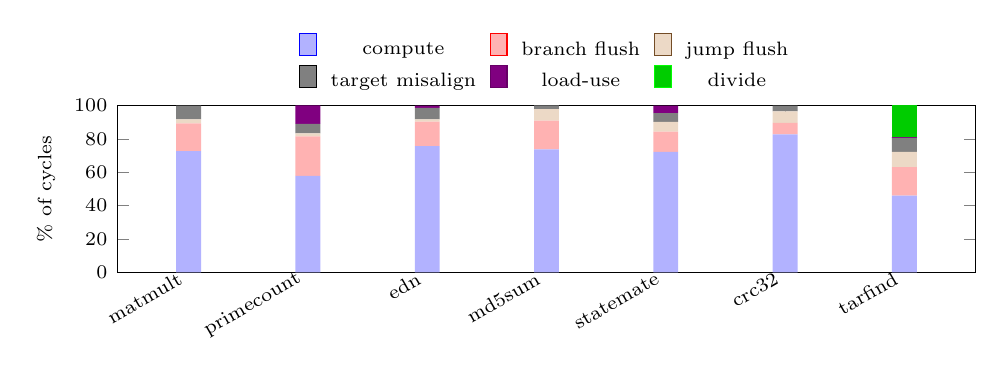
\begin{tikzpicture}
\begin{axis}[
  ybar stacked, bar width=9pt,
  width=1.03\columnwidth, height=3.7cm,
  ymin=0, ymax=100,
  ylabel={\% of cycles}, ylabel near ticks,
  symbolic x coords={matmult,primecount,edn,md5sum,statemate,crc32,tarfind},
  xtick=data,
  x tick label style={rotate=30,anchor=east,font=\scriptsize},
  y tick label style={font=\scriptsize},
  ylabel style={font=\scriptsize},
  legend style={font=\scriptsize,at={(0.5,1.02)},anchor=south,
                legend columns=3,draw=none,column sep=3pt},
  every axis plot/.append style={draw=none},
]
\addplot coordinates {(matmult,72.7)(primecount,57.9)(edn,75.7)(md5sum,73.7)(statemate,72.3)(crc32,82.8)(tarfind,46.0)};
\addplot coordinates {(matmult,16.6)(primecount,23.7)(edn,14.7)(md5sum,17.3)(statemate,12.1)(crc32,6.9)(tarfind,17.1)};
\addplot coordinates {(matmult,2.4)(primecount,1.7)(edn,1.4)(md5sum,6.9)(statemate,5.9)(crc32,6.9)(tarfind,9.2)};
\addplot coordinates {(matmult,8.3)(primecount,5.7)(edn,6.9)(md5sum,2.2)(statemate,5.2)(crc32,3.4)(tarfind,8.4)};
\addplot coordinates {(matmult,0)(primecount,11.1)(edn,1.3)(md5sum,0)(statemate,4.5)(crc32,0)(tarfind,0.4)};
\addplot coordinates {(matmult,0)(primecount,0)(edn,0)(md5sum,0)(statemate,0)(crc32,0)(tarfind,19.1)};
\legend{compute,branch flush,jump flush,target misalign,load-use,divide}
\end{axis}
\end{tikzpicture}
\caption{Where the cycles go on CV32E40X. Compute is the IPC${=}1$ ideal;
everything above it is a stall the manual documents. Control flow costs 14--26\%
on every kernel, and target misalignment alone costs 2.2--8.4\% while needing no
hardware change at all. \texttt{tarfind} is the exception, dominated by divide
latency.}
\label{fig:breakdown}
\end{figure}

Microarchitecture-aware instruction-set-extension (ISE) design for RISC-V has
been studied before, reporting up to $2.47\times$ on Embench and
MiBench~\cite{rezunov}. Our emphasis differs in two respects. First, the estimate
here comes from a model of one specific target pipeline, taken from that core's
published documentation rather than fitted to results, and checked against the
core's own RTL before any of its recommendations are trusted. Second, we cost the
mechanism by which a custom instruction attaches to the core, which turns out to
decide which candidates can pay at all. The work continues
PARISCV~\cite{pariscv1}, a profiler for application-specific RISC-V
optimisation, replacing its estimate with one a candidate can be scored against
before any hardware for it exists. This paper reports that validation and what it
then revealed.

\section{Methodology}

\texttt{spike -l} yields a commit trace of the unmodified binary. A Python
model assigns each instruction its documented cost from the CV32E40X or
CV32E40P user manual~\cite{cv32e40x,cv32e40p} and adds documented penalties:
taken-branch and jump flushes, branch-target misalignment, load-use hazards and
\texttt{jalr} data hazards. Costs are \emph{documented, not fitted}; the
CV32E40P model subclasses the CV32E40X model and overrides only the differences
the manuals state, so it doubles as an executable specification of how the two
cores differ. Divide latency is data-dependent
($3+\mathrm{clz}(\mathit{divisor})$), so the model recovers each actual divisor
by replaying register writes from \texttt{spike --log-commits}.

Code layout has to match. A taken branch costs three cycles, or four when its
target is a non-word-aligned, non-compressed instruction, so two builds of
identical C source linked at different addresses genuinely differ: we measured
5{,}844 against 6{,}356 cycles for the same algorithm. Each kernel is therefore
built twice, Spike at a high address and RTL at the boot address, with
\texttt{.text} verified byte-identical before any number is reported. Skip this
and what looks like model error is mostly an artefact of the harness.

Candidate discovery runs on the same trace. The finder enumerates every
straight-line window of up to four instructions, discards any window containing
control flow, and canonicalises the rest by renaming registers to positional
slots, so one computation collapses to a single candidate however it was
allocated. A window survives only if it reads at most \texttt{X\_NUM\_RS}
registers from the register file and leaves exactly one value live out, which is
what one custom instruction can express; values both produced and consumed inside
the window become internal wires and cost nothing. Survivors are then scored with
the same model, credited with the cycles the sequence costs and debited the
cycles their replacement will itself take.

\section{Validation}

Ground truth is Verilator~\cite{verilator} simulation of each core through
\texttt{core-v-verif}, with the measured region bracketed by \texttt{rdcycle}.

\begin{table*}[t]
\centering
\caption{Model versus RTL on seven Embench-IoT kernels at
\texttt{LOCAL\_SCALE\_FACTOR=1}. The model under-predicts slightly and
consistently, by the few cycles of the \texttt{rdcycle} pair that brackets the
measured region.}
\label{tab:val}
\footnotesize
\setlength{\tabcolsep}{6pt}
\begin{tabular}{@{}lrrrrrrr@{}}
\toprule
& & \multicolumn{3}{c}{CV32E40X} & \multicolumn{3}{c}{CV32E40P}\\
\cmidrule(lr){3-5}\cmidrule(lr){6-8}
kernel & instructions & model & RTL & error & model & RTL & error\\
\midrule
\texttt{matmult-int} & 97{,}748      & 134{,}543   & 134{,}545   & 0.00\% & 134{,}543   & 134{,}547   & 0.00\%\\
\texttt{primecount}  & 2{,}273{,}871 & 3{,}927{,}222 & 3{,}927{,}224 & 0.00\% & 3{,}927{,}222 & 3{,}927{,}226 & 0.00\%\\
\texttt{edn}         & 49{,}365      & 65{,}177    & 65{,}179    & 0.00\% & 65{,}177    & 65{,}181    & 0.01\%\\
\texttt{tarfind}     & 53{,}846      & 117{,}147   & 117{,}149   & 0.00\% & 117{,}147   & 117{,}151   & 0.00\%\\
\texttt{md5sum}      & 52{,}607      & 71{,}398    & 71{,}400    & 0.00\% & 71{,}398    & 71{,}402    & 0.01\%\\
\texttt{statemate}   & 1{,}159       & 1{,}604     & 1{,}606     & 0.12\% & 1{,}604     & 1{,}608     & 0.25\%\\
\texttt{crc32}       & 24{,}608      & 29{,}735    & 29{,}737    & 0.01\% & 29{,}735    & 29{,}739    & 0.01\%\\
\bottomrule
\end{tabular}
\end{table*}

Table~\ref{tab:val} gives 14 points at worst 0.25\%, though that number only
means something alongside how we reached it. For most of the project
\texttt{crc32} sat at $+3.45\%$ on \emph{both} cores, and identical error on two
different microarchitectures pointed at shared logic rather than either pipeline.
Instruction length was being inferred from the printed width of the hex encoding,
but \texttt{spike -l} zero-pads compressed encodings to eight digits too, so
every compressed instruction was mis-sized; \texttt{crc32} branches to one at a
misaligned address and was charged a cycle it never paid on all 1{,}023
iterations. Taking length from the encoding's low two bits, as RISC-V defines,
fixed it. We only found it because a newly added kernel produced a 9\% error too
large to write off, which is how latent modelling bugs tend to surface.

\section{Predicting a change before building it}

\begin{table}[t]
\centering
\caption{Predicted versus measured effect of an ISA change. The Zbb row
is cycles saved; the Xpulp rows are speedup.}
\label{tab:predict}
\footnotesize
\setlength{\tabcolsep}{4pt}
\begin{tabular}{@{}llrrr@{}}
\toprule
change & core & predicted & measured & err\\
\midrule
Zbb enabled    & 40X & 3{,}570        & 3{,}669        & $-2.7\%$\\
Xpulp, 1 loop  & 40P & $3.243\times$  & $3.241\times$  & $-0.10\%$\\
Xpulp, matmult & 40P & $1.305\times$  & $1.502\times$  & $+15\%$\\
\bottomrule
\end{tabular}
\end{table}

Zbb is predicted from a baseline trace before the bitmanip hardware is enabled.
Xpulp is harder: Spike cannot execute Xpulp at all, so the extension's binary
cannot be traced. We instead transform the \emph{baseline} trace analytically, converting counted
loops to hardware loops, folding address arithmetic into post-increment
load/store and fusing \texttt{mul}+\texttt{add} into \texttt{p.mac}, then re-cost
the result with the validated model.

We have kept the $+15\%$ outlier rather than dropping it, because the reason it
is wrong is the useful part.
Recompiling for an extension \emph{relays out the code}, and taken-branch cost
depends on target alignment, which the predictor cannot know from the baseline
layout; it therefore emits an explicit uncertainty band rather than false
precision. More fundamentally, Xpulp's largest win on matmult is not fusion but
\emph{induction-variable strength reduction}: GCC restructures index-based
addressing into pointer-walking \emph{because} post-increment exists.
Predicting an ISA extension therefore means modelling the compiler's response to
it, not only the hardware's. That is a real bound on how far a single baseline
trace can be pushed.

\section{Discovering New Instructions}

A candidate finder mines the trace for straight-line sequences worth fusing,
constrained to one live-out result and a bounded number of register-file
sources, and scores each with the same validated model. Four discovered
instructions were added to CV32E40P by decoder edit and measured. All four
computed correctly and every measured saving fell inside its predicted band. On
the idiom kernels they were mined from, one instruction recovered 2{,}048 of
13{,}326 cycles for a \texttt{crc32} table index (15.4\%), 2{,}048 of 16{,}395
for an \texttt{md5sum} variable rotate (12.5\%), 1{,}024 of 10{,}253 for a
\texttt{matmult-int} indexed load (10.0\%), and nothing at all for an
\texttt{edn} fixed shift.

The bands are not hedging. Fusing removes instructions, and with them the
scheduling slack that was hiding a load-use hazard: after recompiling, GCC
rescheduled the shorter loop so a just-loaded value fed directly into the fused
instruction, costing back what the fusion won. One instruction won its full
predicted 2{,}048 cycles and another won zero, by the same mechanism at
different strengths. A point estimate would have been wrong in both directions.

\textbf{The interface, not the arithmetic, sets the granularity.} We
implemented \texttt{pg.mac}, a fused multiply-accumulate, as a CV-X-IF
coprocessor~\cite{cvxif} on CV32E40X. It computes correctly and won
\textbf{zero cycles}: 13{,}321 versus 13{,}321. The offload costs a cycle,
because the result must be registered and handed back over
\texttt{result\_valid}/\texttt{result\_ready}, so the fused instruction retires
in two cycles where \texttt{mul; add} took two. \emph{A two-instruction fusion
across CV-X-IF can never win}; a sequence must be at least three cycles before
offload pays. Feeding the measured two-cycle latency back into the finder pruned
33 nominally viable candidates on \texttt{matmult-int} to 11, all
memory-addressing sequences, which is what Xpulp implements, now derived from
measurement rather than assumed. The same operation \emph{in} the pipeline
(\texttt{p.mac}) costs one cycle, identical to \texttt{add}. This is the
clearest evidence for why Xpulp lives in the decoder and why CV-X-IF suits
coarse-grained offload instead.

\textbf{Free cycles with no hardware.} Branch-target misalignment costs
2.2--8.4\% of all cycles across our kernels. On \texttt{edn} that is 4{,}465
cycles, larger than the 3{,}669 cycles won by enabling the entire bitmanip
extension. All it needs is alignment from the compiler or linker.

\section{Conclusions and Future Work}

A cycle model taken from published pipeline documentation rather than fitted to
measurements predicted real-core cycle counts on two OpenHW cores to within
0.25\%, and that was accurate enough to settle design questions before the
hardware existed: whether to enable Zbb, what Xpulp would be worth, and which
four custom instructions to add. Those instructions recovered 10--15\% of their
kernels' cycles wherever they paid at all, and Xpulp reached $3.24\times$ on a
single loop. The result we did not anticipate is that the
interface, not the arithmetic, sets the smallest fusion worth building. Two
upstream bugs were found and patched on the way, one leaving every CV32E40X
load and store carrying zero in \texttt{core-v-verif}'s Verilator wrapper, the
other mis-ordering nested hardware-loop registers in the PULP GCC fork.

This remains work in progress. The model covers in-order pipelines with a
zero-wait-state memory; extending it to a cached core is ongoing. The
granularity result above also points at its own next step: since a sequence must
exceed roughly three cycles before CV-X-IF offload pays, the candidates the
finder retains after calibration are exactly the coarse ones, and the natural
target for them is a PULP-style accelerator such as RedMulE~\cite{redmule},
which attaches over CV-X-IF itself. Routing a candidate to an accelerator rather
than an instruction requires predicting the \emph{residual} cost left on the
core (data marshalling, configuration and synchronisation), which is the same
quantity the stall breakdown already reports. Code, patches and every number
above: \url{https://github.com/ashuthosh-mr/mouna}.

\section*{Acknowledgment}

The cycle models, the candidate finder, the custom-instruction RTL and the
drafting of this paper were produced with the assistance of an AI coding
assistant (Anthropic Claude), directed by the author. Every performance figure
reported here was measured by the author on RTL simulation of the cores named,
and the author is solely responsible for the content and for any errors.

\balance
\begin{thebibliography}{9}
\small
\bibitem{embench} J.~Bennett \emph{et al.}, ``Embench: A Modern Embedded
Benchmark Suite,'' \url{https://www.embench.org}.
\bibitem{rezunov} E.~Rezunov, N.~Zurstra{\ss}en, L.~M.~Reimann and R.~Leupers,
``Automatic Microarchitecture-Aware Custom Instruction Design for RISC-V
Processors,'' arXiv:2509.15782, 2025.
\bibitem{cv32e40x} OpenHW Group, \emph{CV32E40X User Manual}.
\bibitem{cv32e40p} OpenHW Group, \emph{CV32E40P User Manual}.
\bibitem{cvxif} OpenHW Group, \emph{CORE-V eXtension Interface (CV-X-IF)
Specification}.
\bibitem{verilator} W.~Snyder, ``Verilator,'' \url{https://verilator.org}.
\bibitem{redmule} Y.~Tortorella, L.~Bertaccini, L.~Benini, D.~Rossi and
F.~Conti, ``RedMulE: A Mixed-Precision Matrix-Matrix Operation Engine for
Flexible and Energy-Efficient On-Chip Linear Algebra and TinyML Training
Acceleration,'' arXiv:2301.03904, 2023.
\bibitem{xpulp} M.~Gautschi \emph{et al.}, ``Near-Threshold RISC-V Core With
DSP Extensions for Scalable IoT Endpoint Devices,'' \emph{IEEE Trans. VLSI
Syst.}, 2017.
\bibitem{pariscv1} Spoorthi~S., M.~R.~Ashuthosh, Bharadhwaj~K., V.~Reddy and
M.~Purnaprajna, ``PARISCV: A RISC-V Profiler for Application-Specific Hardware
Optimization,'' in \emph{Proc. IEEE 32nd Int. Conf. High Performance Computing,
Data and Analytics Workshop (HiPCW)}, 2025, pp.~303--304.
\end{thebibliography}

\end{document}
